

\documentclass[10pt]{article}

\usepackage{fullpage}
\usepackage{graphicx}
\usepackage{mathtools}
\usepackage{setspace}
\usepackage{mdwlist}
\usepackage[center]{caption}
\onehalfspacing

\begin{document}
\title{Project Proposal\\Augmented Reality Image Processing System}
\author{Logan P. Williams \& Jos\'{e} E. Cruz Serrall\'{e}s}
\date{November 15, 2011}
\maketitle



\section*{Abstract}
We will implement an augmented reality system that can overlay a digital image on video of a real world environment. We begin by reading NTSC video from a video camera and storing it in ZBT SRAM. A picture frame with colored markers on the corners is held in front of the camera. We then perform chroma-based object recognition to locate the co-ordinates of the corners. Using these co-ordinates, we apply a low-pass filter and a projective transformation to project an image onto the dimensions of the picture frame. We then output VGA video of the original captured image, with the processed image overlayed on top of the frame. The overlayed image (the ``augmentation'') can be arbitrary. When this image is the frame of video that was previously displayed, we call the system ``recursive'', as we obtain the same image contained within itself.

\tableofcontents


\section{Top-Level Block Diagram}
\begin{figure}[h!]
\centering
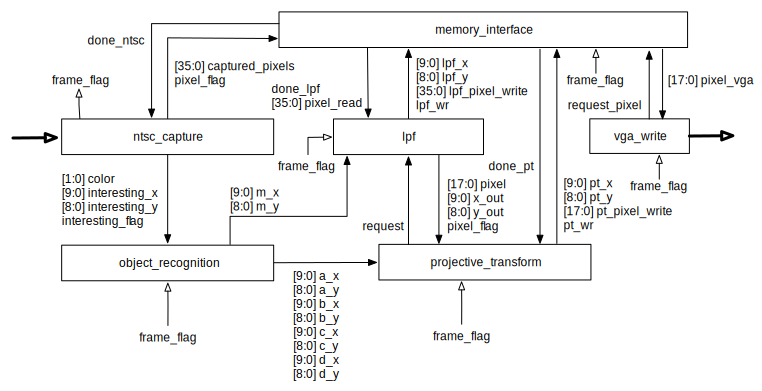
\includegraphics[width=\textwidth]{block_diagram_with_wires.png}
\caption{\emph{The block diagram of the augmented reality system.}}
\end{figure}
\section{Submodules}
% 1) inputs & outputs
% 2) some indication of its complexity and level of performance
%	a) number and type of arithmetic operations
%	b) size of internal memories
%	c) required throughput
%	etc.
% 3) how the module will be tested
% 4) who will be writing the module
\subsection{NTSC Capture (Logan)}
The NTSC capture module is almost unmodified from the code provided by 6.111. It takes as input an NTSC video signal, and writes pixels into ZBT Memory.

There are two modifications. The first allows the module to capture and store color data, converting it from Y/Cr/Cb to H/S/V. The second modification is added to support object recognition. When the Capture module sees a pixel of a hue that matches the target (blue, green, red, and yellow), it sends information (the color and its X/Y location) to the Object Recognition module. It also outputs a flag that goes high when the entire frame has been captured.

This module can be tested by connecting it to the VGA output module and ensuring that the video output is the image seen by the video camera.

\subsection{Memory Interface (Jos\'{e})}
% Jose
The Memory Interface handles the interaction between all of the other modules and the two ZBT Memory blocks, which house the four images that the modules use for capturing, displaying, and processing. Ideally, BRAM would have been used, but the number of pixels that we would like to store vastly exceeds BRAM capacity. Unlike BRAM, each ZBT Memory block can only handle one read or write operation per cycle, causing memory access to be the main bottleneck of our system. As such, we will store only the six most significant bits of each component of every pixel, allowing us to store two pixels per address and to reduce the number of memory accesses in our system by a factor of two.

Memory Interface will allocate two images per memory block. These four images will be (1) "capture", the image being captured from NTSC; (2) "display", the image being displayed in the VGA; (3) "processing", the image that will be processed by the LPF and projected by projective\_transform; and (4) "next\_display", the image to which projective\_transform will write and the next image that will be displayed. Every image refresh (1/30 seconds), the previous "next\_display" will become the next "display", the previous "display" will become the next "processing", the previous "capture" will become the next "next\_display", and the previous "processing" will become the next "capture". These location shifts will be transparent to the other modules. Read and write requests from vga\_write and ntsc\_capture will be given priority over requests from other modules.

The inputs to Memory Interface are (1) frame\_flag, which signals when to shift; (2) two pixels from NTSC capture; (3) two (x,y) pairs, one from LPF and one from projective\_transform; (4) two pixels from LPF; (5) one pixel from projective\_transform; and (6) request flags and (7) write flags from other submodules. The outputs from Memory Interface are (1) done flags; (2) one pixel to vga\_write; and (3) two pixels to LPF.

The Memory Interface module will be tested in stages. Initially, basic read and write functionality will be assessed in simulation and then on the FPGA. Once we have written and read information from the ZBT RAM successfully, we will attempt to write, read, and display an image. Finally, all of the logic pertaining to handling read and write requests from all the modules simulatenously will be written, tested using extensive testbenches, and finally tested on an FPGA with dummy modules. All of this testing should avoid help us avoid headaches during final integration.

\subsection{Object Recognition (Logan)}
The {\tt object\_recognition} module collects ``interesting'' pixels located by the NTSC Capture module, and calculates the center of mass of each color, to find the location of the corners of the picture frame.

It takes as inputs (1) the color of a detected pixel, (2) a flag that goes high for one clock cycle when a pixel is detected, (3) the X/Y coordinates of the pixel, and (4) a flag that goes high when a new frame is beginning. It produces as output four sets of X/Y coordinates, one for the center of mass of each color.

The center of mass will be calculating with a simple linear weighting scheme, averaging the X and the Y coordinate for each pixel independently to find the center X/Y location, which are used by the {\tt lpf} and the {\tt projective\_transfom} module. This module can be tested with a simple test bench that provides some sample pixel locations, and tests to see if the module computes the center of mass correctly.

\subsection{ArbiLPF (Jos\'{e})}
% Jose
The inputs to ArbiLPF are (1) the downsampling coefficient (M), (2) the index of the pixel in displayed image to be filtered given this downsampling factor, (3) the set of pixels around the filtered pixels required for filtering, and (4) the pulse from the memory module. ArbiLPF applies a two-dimensional low-pass filter to this pixel by using surrounding pixels to calculate the convolution sum. The radial cutoff frequency of this 2D filter is of \( \frac{\pi}{M} \), in order to avoid aliasing in the ArbiSkew module. The outputs of ArbiLPF are (1) the pixel values of the output of the lowpassed version of this image, sampled at the given index, and (2) the indices of the set of pixels that are needed for filtering.

Based on the downsampling factor M, the filter will select a set of coefficients from a lookup table and convolve the image values with these coefficients. This table of coefficients will correspond to the coefficients of 2D extrapolations of 1D FIR Parks-McClellan filters with cutoff frequencies of \( \frac{\pi}{M} \). Due to the limited number of multipliers on the FPGA and the single-input, single-output of the RAM module, these 2D filters will be constrained to have at most 16 coefficients, which constrains the one-dimensional filters to have at most 4 coefficients. Due to these constraints, the ripple and transition width specifications of the 1D filters will have to be lax. The radial symmetry of these 2D filters will be exploited to reduce the number of required multiplications by a factor of 4, to at most 4 multiplications per color per pixel or 12 multiplications per pixel.

Due to the single-input, single-output nature of the RAM, the clock frequency of this module will have to be greater than 80MHz. Given relatively little contention from other blocks, ArbiLPF will elapse at least 9 cycles at 90MHz per pixel, yielding a latency of 0.03072 seconds or a little less than one NTSC refresh period. ArbiLPF will also have to perform roughly eight additions per cycle, but the timing constraints imposed by these additions are negligible when compared to the multiplications.

ArbiLPF will be tested by crafting a testbench module that accepts an arbitrary 640x480 image and outputs the output of the filter. Initially, an image with an impulse at the center will be used, which ideally should cause the filter to output the filter coefficients that are used. As basic functionality is tested, more complicated images will be used. Eventually, complex images will be processed both with the testbench and with MATLAB and will be compared using the 2D Fourier plots of these two outputs.

\subsection{Projective Transform (Logan)}
% Logan
The inputs to {\tt projective\_transform} are (1) the pixel value last produced by {\tt lpf}, (2) a flag signal held high for one clock signal when {\tt lpf} has processed a new pixel, (3) the four coordinates of the corners of the frame provided by the {\tt object\_recognition} module, and (4) a signal when a new frame is beginning.

The outputs from {\tt projective\_transform} are (1) a request to {\tt lpf} for a new pixel, (2) the X/Y coordinates of the transformed pixel, (3) the transformed pixel value, and (4) a flag indicating that a new pixel is to be written.

This function maps the original rectangular image to any convex quadrilateral, provided that all sides of the destination quadrilateral are shorter than the original, which is inherent in the overall system. A graphic representation of the transformation is shown in Figure 2, on the next page.

\begin{figure}[h!]
\centering
\includegraphics[width=0.65\textwidth]{arbiskew_graphic.png}
\caption{\emph{A visual representation of the result of the {\tt projective\_transform} module. Input is on the left, a possible output, for four coordinates $A\prime$, $B\prime$, $C\prime$, and $D\prime$ is on the right.}}
\end{figure}

Mathematically, the algorithm works as follows:
\begin{enumerate*}
\item Calculate the distance of line $\overline{A\prime D\prime}$ and assign it to $d_{ad}$.
\item Do the same for $\overline{B\prime C\prime}$ and assign it to $d_{bc}$.
\item Create two ``iterator points,'' point $I_A$ and $I_B$ initially located at $A\prime$ and $B\prime$.
\item Let $o_x = 0$ and $o_y = 0$
\item Calculate the distance between the iterator points, assign it to $d_i$.
\item Create a third iterator point, $I_C$ at the location $I_A$.
\item Assign the pixel value of $I_C$ to pixel $(o_x, o_y)$ in the original image.
\item Move $I_C$ along line $\overline{I_A I_B}$ by an amount $= \frac{d_i}{width_{original}}$.
\item Increment $o_x$.
\item Repeat steps 7--9 until $I_C = I_B$.
\item Move $I_A$ along line $\overline{A\prime D\prime}$ by an amount $= \frac{d_{ad}}{height_{original}}$.
\item Move $I_B$ along line $\overline{B\prime C\prime}$ by an amount $= \frac{d_{bc}}{height_{original}}$.
\item Increment $o_y$.
\item Repeat steps 5--13 until $I_A = D\prime$ and $I_B = C\prime$.
\end{enumerate*}

This algorithm needs a relatively small number of multiplications, just two per pixel in the original image, and four per line in the original image. There is also a square root that is needed once per line, which will be implemented with an iterative algorithm.

The {\tt projective\_transform} module can be tested by creating a test bench that provides a series of test pixels as input. The output generated in ModelSim by {\tt projective\_transform} can then be compared with the output generated by a MATLAB implementation of the algorithm described above.

\subsection{VGA Write (Jos\'{e})}
% Jose
The VGA Write section is straightforward and will basically be a clone of the VGA code used in Lab 2 (Pong). Essentially, the output will be refreshed at a rate of 60Hz and output at a resolution of 640x480 pixels. This module will read the pixel values from displayed image and assign it based on the hcount and vcount variables, which will be incremented accordingly. This module will be tested by loading a standardized image to memory and verifying whether VGA Write displays this image properly on the monitor.

\section{External Components}
We will be using two standard external components: an video camera that provides NTSC composite video out, to be provided by the 6.111 staff, and a VGA display.

\section{Project Deadlines}
% A calendar-like view of what deadlines we'll set ourselves, when everything should be operational, etc. Maybe this could be collapsed into the submodules section
\begin{itemize}
\item 11-11-2011 - Finalized Block Diagram
\item 11-18-2011 - First draft of ArbiLPF, ArbiSkew, and ZBT Memory written
\item 11-22-2011 - VGA Write and NTSC Capture first drafts written; ArbiLPF, ArbiSKEW, ZBT Memory fully tested
\item 11-30-2011 - NTSC Capture and VGA Write fully tested; start of full integration
\item 12-05-2011 - Full integration
\item 12-12-2011 - Final report due
\end{itemize}

\end{document}
